\documentclass{article}
\usepackage{graphicx} % Required for inserting images
\usepackage{amsmath}
\usepackage{amssymb} % used for math symbols
\usepackage{mathtools}

\title{Computer Grafik Blatt 2}
\date{May 2023}

\begin{document}

\maketitle

\section*{Aufgabe 1:}

\subsection*{a)}

\subsubsection*{Mittelpunkt:}
\[
    \begin{pmatrix}
            4 \\
            2 \\
            -6 \\
            1
    \end{pmatrix}
\]
\subsubsection*{Eckpunkte:}
\[
    luv:
    \begin{pmatrix}
            0 \\
            -2 \\
            -2 \\
            1
    \end{pmatrix}
    ruv:
    \begin{pmatrix}
            8 \\
            -2 \\
            -2 \\
            1
    \end{pmatrix}
    ruh:
    \begin{pmatrix}
            8 \\
            -2 \\
            -10 \\
            1
    \end{pmatrix}
    luh:
    \begin{pmatrix}
            0 \\
            -2 \\
            -10 \\
            1
    \end{pmatrix}
    \]\[
    loh:
    \begin{pmatrix}
            0 \\
            6 \\
            -10 \\
            1
    \end{pmatrix}
    roh:
    \begin{pmatrix}
            8 \\
            6 \\
            -10 \\
            1
    \end{pmatrix}
    rov:
    \begin{pmatrix}
            8 \\
            6 \\
            -2 \\
            1
    \end{pmatrix}
    lov:
    \begin{pmatrix}
            0 \\
            6 \\
            -2 \\
            1
    \end{pmatrix}
\]
Es wird unterschieden in links-rechts, unten-oben und vorne-hinten.

\subsubsection*{Projektionen:}
\[
luv' = \begin{pmatrix}
        1&0&0&0\\
        0&1&0&0\\
        0&0&1&0\\
        0&0&-1&0
\end{pmatrix}
\begin{pmatrix}
        0\\-2\\-2\\1
\end{pmatrix}
=
\begin{pmatrix}
 0\\-2\\-2\\2
\end{pmatrix}
\Rightarrow
\begin{pmatrix}
 0\\-1\\-1\\1
\end{pmatrix}
\]
\[
ruv' = \begin{pmatrix}
        1&0&0&0\\
        0&1&0&0\\
        0&0&1&0\\
        0&0&-1&0
\end{pmatrix}
\begin{pmatrix}
        8\\-2\\-2\\1
\end{pmatrix}
=
\begin{pmatrix}
 8\\-2\\-2\\2
\end{pmatrix}
\Rightarrow
\begin{pmatrix}
 4\\-1\\-1\\1
\end{pmatrix}
\]
\[
ruh' = \begin{pmatrix}
        1&0&0&0\\
        0&1&0&0\\
        0&0&1&0\\
        0&0&-1&0
\end{pmatrix}
\begin{pmatrix}
        8\\-2\\-10\\1
\end{pmatrix}
=
\begin{pmatrix}
 8\\-2\\-10\\10
\end{pmatrix}
\Rightarrow
\begin{pmatrix}
 0,8\\-0,2\\-1\\1
\end{pmatrix}
\]
\[
luh' = \begin{pmatrix}
        1&0&0&0\\
        0&1&0&0\\
        0&0&1&0\\
        0&0&-1&0
\end{pmatrix}
\begin{pmatrix}
        0\\-2\\-10\\1
\end{pmatrix}
=
\begin{pmatrix}
 0\\-2\\-10\\10
\end{pmatrix}
\Rightarrow
\begin{pmatrix}
 0\\-0,2\\-1\\1
\end{pmatrix}
\]
\[
loh' = \begin{pmatrix}
        1&0&0&0\\
        0&1&0&0\\
        0&0&1&0\\
        0&0&-1&0
\end{pmatrix}
\begin{pmatrix}
        0\\6\\-10\\1
\end{pmatrix}
=
\begin{pmatrix}
 0\\6\\-10\\10
\end{pmatrix}
\Rightarrow
\begin{pmatrix}
 0\\0,6\\-1\\1
\end{pmatrix}
\]
\[
roh' = \begin{pmatrix}
        1&0&0&0\\
        0&1&0&0\\
        0&0&1&0\\
        0&0&-1&0
\end{pmatrix}
\begin{pmatrix}
        8\\6\\-10\\1
\end{pmatrix}
=
\begin{pmatrix}
 8\\6\\-10\\10
\end{pmatrix}
\Rightarrow
\begin{pmatrix}
 0,8\\0,6\\-1\\1
\end{pmatrix}
\]
\[
rov' = \begin{pmatrix}
        1&0&0&0\\
        0&1&0&0\\
        0&0&1&0\\
        0&0&-1&0
\end{pmatrix}
\begin{pmatrix}
        8\\6\\-2\\1
\end{pmatrix}
=
\begin{pmatrix}
 8\\6\\-2\\2
\end{pmatrix}
\Rightarrow
\begin{pmatrix}
 4\\3\\-1\\1
\end{pmatrix}
\]
\[
lov' = \begin{pmatrix}
        1&0&0&0\\
        0&1&0&0\\
        0&0&1&0\\
        0&0&-1&0
\end{pmatrix}
\begin{pmatrix}
        0\\6\\-2\\1
\end{pmatrix}
=
\begin{pmatrix}
 0\\6\\-2\\2
\end{pmatrix}
\Rightarrow
\begin{pmatrix}
 0\\3\\-1\\1
\end{pmatrix}
\]

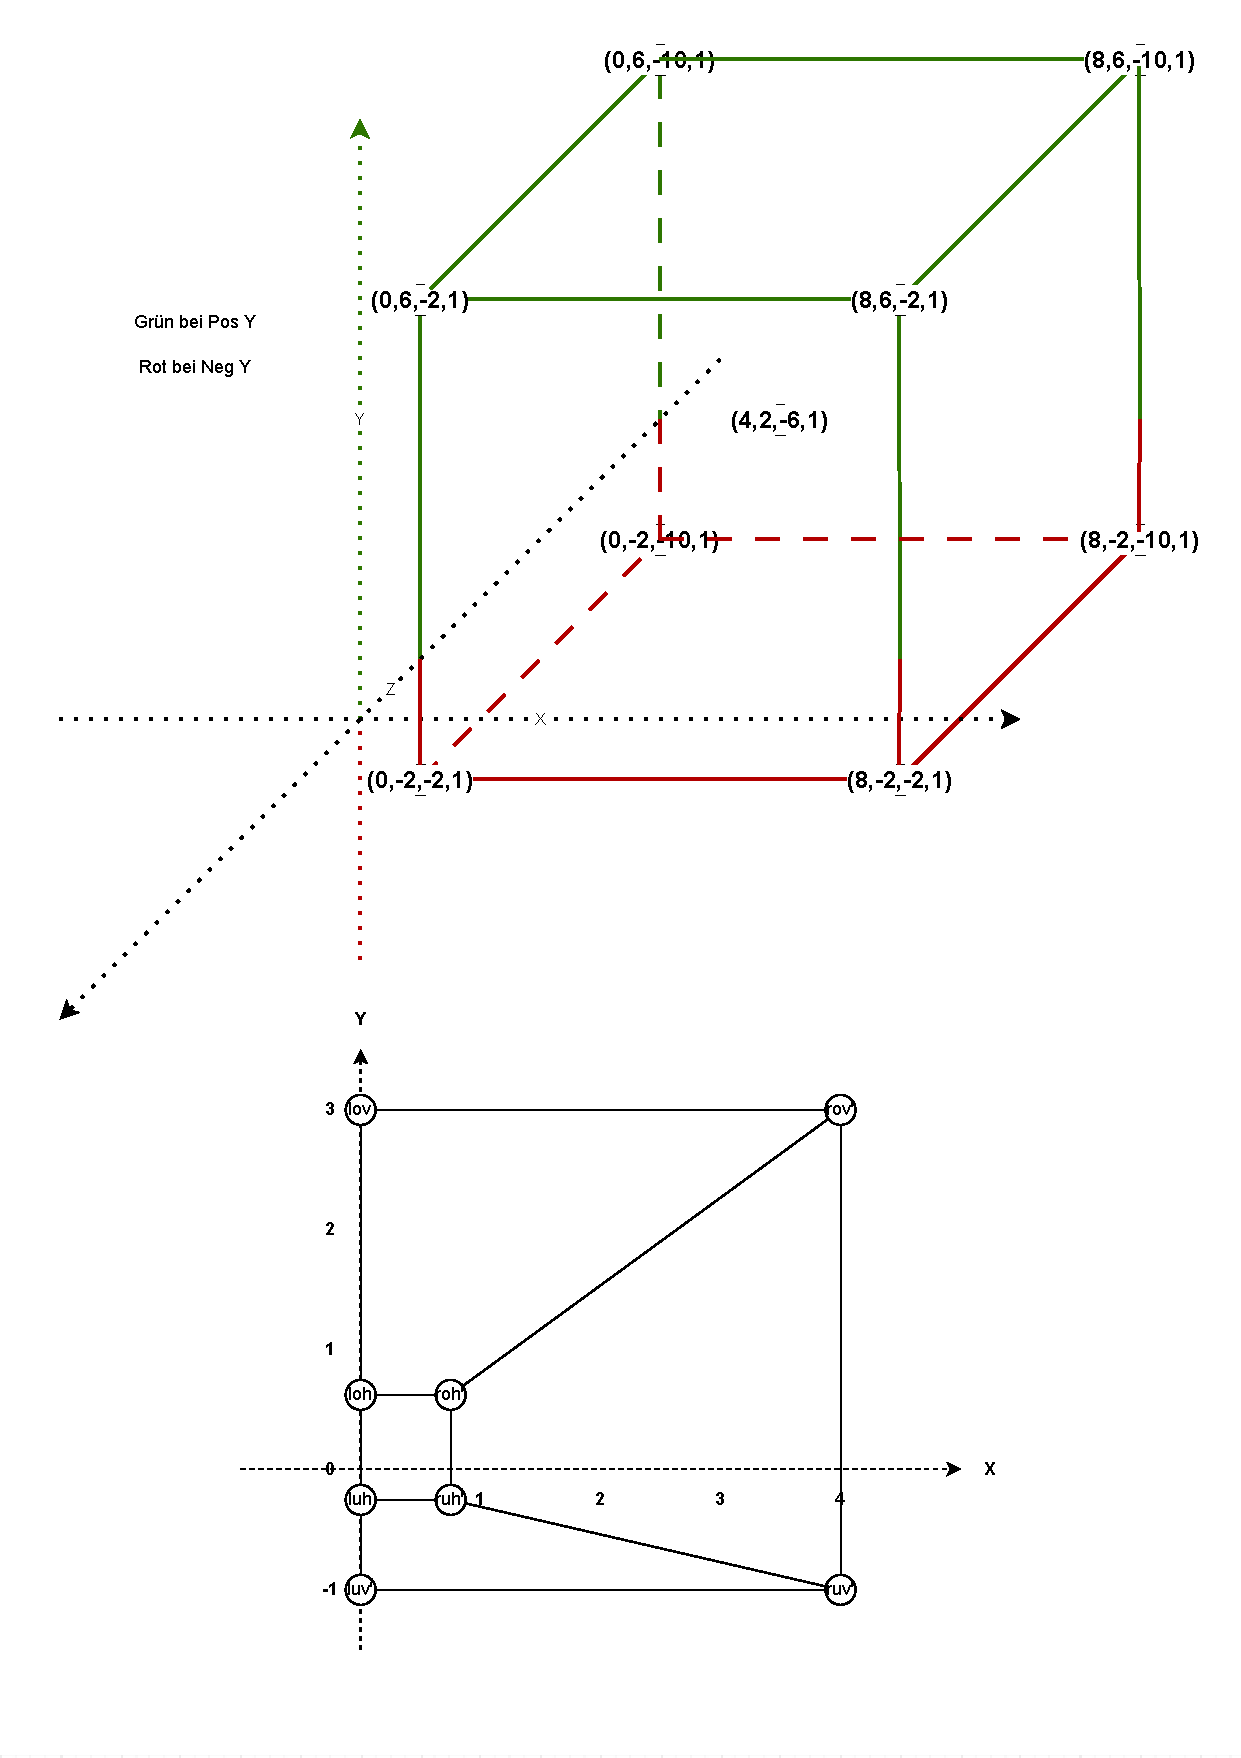
\includegraphics[width=1.2\textwidth,keepaspectratio]{CG_Blatt2_bild_und_drawio.pdf}

\subsection*{b)}

\begin{enumerate}
    \item Zuerst überprüfen wir ob Richtung $\overrightarrow{d}$ und up-Vektor $\overrightarrow{u}$senkrecht zueinander sind:
    \[
    d^Tu= 
    \begin{pmatrix}
    -\frac{4}{5}&0&\frac{3}{5}
    \end{pmatrix}
    \begin{pmatrix}
    0\\1\\0
    \end{pmatrix}
    = 0 \;\checkmark
    \]
    \item
    Danach bestimmen wir $\overrightarrow{r}$:
    \[
    \overrightarrow{r}=\overrightarrow{d}\times\overrightarrow{u}=
    \begin{pmatrix}
    0\cdot0-\frac{3}{5}\cdot1\\
    \frac{3}{5}\cdot0-(-\frac{4}{5})\cdot 0\\
    -\frac{4}{5}\cdot 1 - 0\cdot 0
    \end{pmatrix}
    =
    \begin{pmatrix}
    -\frac{3}{5}\\
    0\\
    -\frac{4}{5}
    \end{pmatrix}
    \]
    \item
    Dann bestimmen wir $-r^Tc,-u^Tc$ und $d^Tc$:
    \[
    -r^Tc=
    \begin{pmatrix}
    \frac{3}{5}&0&\frac{4}{5}&0
    \end{pmatrix}
    \begin{pmatrix}
    3\\0\\2\\1
    \end{pmatrix}
    = \frac{17}{5}
    \]
    \[
    -u^Tc =
    \begin{pmatrix}
    0&-1&0&0
    \end{pmatrix}
    \begin{pmatrix}
    3\\0\\2\\1
    \end{pmatrix}
    = 0
    \]
    \[
    d^Tc=
    \begin{pmatrix}
    -\frac{4}{5}&0&\frac{3}{5}&0
    \end{pmatrix}
    \begin{pmatrix}
    3\\0\\2\\1
    \end{pmatrix}
    =-\frac{6}{5}
    \]
    \item 
    Am Ende ergibt sich aus der Formel im Kompaktskritp:
    \[
    M_{LookAt_{\overrightarrow{r},\overrightarrow{u},-\overrightarrow{d},c}}=
    \begin{pmatrix}
    -\frac{3}{5}&0&-\frac{4}{5}&\frac{17}{5}\\
    0&1&0&0\\
    \frac{4}{5}&0&-\frac{3}{5}&-\frac{6}{5}\\
    0&0&0&1
    \end{pmatrix}
    \]
\end{enumerate}

\subsection*{c)}

\begin{enumerate}
    \item 
    \[
    ||\overrightarrow{v}||=\sqrt{\cos{\alpha}\cdot v^T\cdot v} = 
    \sqrt{1\cdot
    \begin{pmatrix}
     -5&4&-20
    \end{pmatrix}
    \begin{pmatrix}
     -5\\4\\-20
    \end{pmatrix}}
    = \sqrt{441}=21
    \]
    
    \item
    \[
    v^Tw=\cos{\alpha}\cdot ||v||\cdot||w|| = 
    \begin{pmatrix}
     0&8&8
    \end{pmatrix}
    \begin{pmatrix}
     0\\0\\-2
    \end{pmatrix}
    = -16
    \]\[
    ||v||=\sqrt{0^2 + 8^2 + 8^2}=8\sqrt{2}
    \]\[
    ||w||= \sqrt{0^2 +0^2 +(-2)^2}=2
    \]\[
    \cos{\alpha}\cdot ||v||\cdot||w|| = \cos{\alpha}\cdot 4\sqrt{2}\cdot2 = -16 | \div 2 | \div 8\sqrt{2}
    \]\[
    \cos{\alpha} = -\frac{\sqrt{2}}{2} = 135^\circ
    \]
    
    \item 
    \[
    \overrightarrow{x}= \overrightarrow{v}\times \overrightarrow{w}=
    \begin{pmatrix}
     v_2w_3 -v_3w_2\\
     v_3w_1-v_1w_3\\
     v_1w_2-v_2w_1
    \end{pmatrix}
    =
    \begin{pmatrix}
    36\cdot1-(-4)\cdot1\\
    (-4)\cdot1-6\cdot1\\
    6\cdot1-36\cdot1
    \end{pmatrix}
    =
    \begin{pmatrix}
    40\\
    -10\\
    -30
    \end{pmatrix}
    \]
    
    \item
    Gesucht ist $\overrightarrow{v}$, sodass $\overrightarrow{v} \cdot \overrightarrow{w} = 0$.
    \[
        \overrightarrow{v} \cdot \overrightarrow{w} = v_1 \cdot w_1 + v_2 \cdot w_2 + v_3 \cdot w_3 = 0
    \]
    Da $\overrightarrow{w} = ((-1,8,7) - \overrightarrow{v})$ folgt daraus in die Formel eingesetzt
    \[
        \begin{aligned}
            &v_1 \cdot (-1 - v_1) + v_2 \cdot (8 - v_2) + v_3 \cdot (7 - v_3) &&= 0 \\
            &\Leftrightarrow -v_1^2 - v_1 - v_2^2 - v_3^2 + 8 v_2 + 7 v_3 &&= 0
        \end{aligned}
    \]
    
    Durch die möglichen Lösungen für die Gleichung ergeben sich dann beispielsweise folgende Vektoren für $\overrightarrow{v}$:
    \[
        \begin{pmatrix}
            0 \\ 0 \\ 0
        \end{pmatrix},
        \begin{pmatrix}
            0 \\ 0 \\ 7
        \end{pmatrix},
        \begin{pmatrix}
            3 \\ 0 \\ 3
        \end{pmatrix},
        \begin{pmatrix}
            3 \\ 0 \\ 4
        \end{pmatrix},
        \begin{pmatrix}
            2 \\ 0 \\ 6
        \end{pmatrix},
        \begin{pmatrix}
            -1 \\ 0 \\ 7
        \end{pmatrix} \dots
    \]
\end{enumerate}

\end{document}
